\documentclass[superscriptaddress,floatfix,reprint,amssymb, amsmath,aps, pre]{revtex4-1}
\usepackage[utf8]{inputenc}
\usepackage[T1]{fontenc}
\usepackage{amsmath}
\usepackage{amsfonts}
\usepackage{amssymb}
\usepackage{graphicx}
\usepackage{bm}
\usepackage{grffile} %Allows figure file names with periods
\usepackage{xr} %use for supplementary material
\usepackage{xcolor}
\usepackage{epsfig}
\usepackage{graphicx}
\usepackage{amssymb}
\usepackage{enumerate}
\usepackage{enumitem}
\usepackage{float}
%\usepackage{lipsum}
% \usepackage{mathtools}
% \usepackage{subcaption}
% \usepackage{relsize}
\usepackage{listings}
% \usepackage{color}
\usepackage{hyperref}
% \usepackage{relsize}
% \usepackage{commath}
\usepackage{dirtytalk}
\usepackage{titlesec}
\usepackage{relsize}
\usepackage{amsmath}
\usepackage{breqn}

\newcommand{\C}{\mathbb{C}}
\newcommand{\I}{\mathbb{I}}
\newcommand{\R}{\mathbb{R}}
\newcommand{\N}{\mathbb{N}}
\newcommand{\K}{\mathbb{K}}

\newcommand{\rd}{\textrm{d}}

\newcommand{\bc}{\textbf{c}}
\newcommand{\bbf}{\textbf{f}}
\newcommand{\bg}{\textbf{g}}
\newcommand{\bu}{\textbf{u}}
\newcommand{\bv}{\textbf{v}}
\newcommand{\bw}{\textbf{w}}
\newcommand{\bx}{\textbf{x}}
\newcommand{\by}{\textbf{y}}

\externaldocument[supp-]{CC_OA_comparison_supplementary}
\newcommand{\diag}[1]{\textrm{diag}\left(#1\right)}
\newcommand{\dbyd}[1]{\frac{\rd}{\rd#1}}
\newcommand{\re}[1]{\textrm{Re}\left(#1\right)}
\newcommand{\imag}[1]{\textrm{Im}\left(#1\right)}
\newcommand{\trace}[1]{\textrm{tr}\left(#1\right)}
\newcommand{\deriv}[2]{\dfrac{ d #1}{ d #2}}
\newcommand{\fn}[1]{f_{ #1}}
\newcommand{\aee}{\alpha_\epsilon}
\newcommand{\tee}{\theta_\epsilon}
\newcommand{\uee}{u_\epsilon}

\renewcommand{\labelenumii}{\theenumii}
\renewcommand{\theenumii}{\theenumi.\arabic{enumii}.}
\newcommand\numberthis{\addtocounter{equation}{1}\tag{\theequation}}
\graphicspath{{Figures/}}

\titlespacing\section{0pt}{12pt plus 4pt minus 2pt}{0pt plus 2pt minus 2pt}
\titlespacing\subsection{0pt}{12pt plus 4pt minus 2pt}{0pt plus 2pt minus 2pt}
\titlespacing\subsubsection{0pt}{12pt plus 4pt minus 2pt}{0pt plus 2pt minus 2pt}

\hypersetup{
    colorlinks = false,
    linkbordercolor = {white},
    citebordercolor = {white},
}

\newcommand{\squeezeup}{\vspace{-3mm}}

\begin{document}
{
    \title{Control methods for Inverted Rotary Pendulum}
    \author{Ankith Anil Das\\
    470485327}

    \maketitle

    \section{Introduction}{
        Inverted pendulum control is one of the fundamental but interesting problems in the field of control theory. This system consists of a rotary arm controlled by an input torque, \(\tau\) , and an unactuated pendulum connected to the arm at a pivot joint . Different control algorithms are applied for solving swing-up control and stabilization problems. The equations of motion are non-linear. Therefore, they can be linearized at an operating point to carry out proper solutions[6]. 

        This model has been significantly used in applications such as position control, aerospace vehicle controls and robotics \cite{wolenski_controller_2011}. These applications can be found in transport machines that need to balance objects, in systems that support walking for patients, in robots that are used in domestic and industrial use and in object transport using drones \cite{kafetzis_inverted_2017}. This paper uses stabilization controllers to design a closed-loop pole placement. 

        This paper proposes design of controller for inverted pendulum system. Stabilization controllers were designed based on pole placement technique. Pole placement technique is used to get desired characteristics for the closed loop system. Pole placement is a well-known design technique that provides practical feedback gain to enable the closed-loop stable and high performance design of systems \cite{noauthor_lqr_nodate}. This technique also produces robustness property even in the face of certain gain.

        The first step was to determine the equations of motion for the inverted pendulum, using the Euler-Lagrange equations. It was then continued with finding a linearized model that approximated the original nonlinear system’s behavior around the equilibrium located on the upright vertical position. Using the linearized model, we designed a state feedback controller and observer by desired pole placement. Then we proceeded to make a swing up controller to bring the pendulum to a vertically upright position. Finally, we looked at a way to design a non-linear observer which can observe the system at all state values. 
    }
    \section{System Description}{
        The Quanser SRV02 is a rotary servo plant attached to a pendulum arm, a physical model of such a system is presented in Fig. \ref{fig:rotarySystem}. The system introduced in this report consists of two components, a servo module and a rotary module.  The servo module consists of a DC servomotor mated with a gearbox of ratio 70:1 and has an input voltage of \(\pm 6\) V and is bolted directly to an aluminium frame for support. The independent output shaft driven by the motor rotates inside of a high-precision ball bearing block to minimize frictional losses. The output position and angle are measured through built in sensors on the output shaft. The second component of the system, the rotary module consists of two links, the first of which is a horizontal link called the rotating arm, and the second being a vertical link called the pendulum. The arm is rotated in the horizontal plane while the pendulum is allowed to move along the radial direction of the motor. This system was chosen as it had a detailed description of parameter values, making the modelling and simulation process more streamlined. Detailed description of the plant can be found at \cite{apkarian_user_2011}. The system parameters are shown in Table. \ref{tab:systemData}.
        \begin{figure}[h!]
            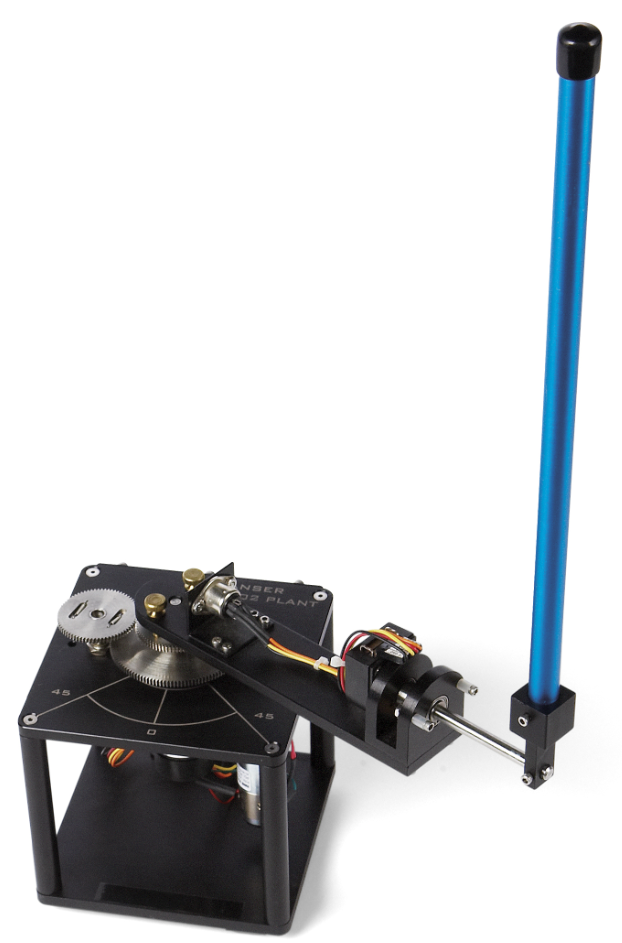
\includegraphics[width = 0.5\linewidth]{systemPic.png}
            \caption{Quanser SRV02 rotary servo plant attached with a pendulum arm}
            \label{fig:rotarySystem}
        \end{figure}
        \begin{table}[h!]
            \caption{Parameters of Rotary Pendulum \cite{apkarian_user_2011} }
            \begin{tabular}{cccc}
                \hline Parameter & Description & Value & Unit \\
                \hline
                $m_{r}$ & Mass of rotary arm & 0.257 & $\mathrm{kg}$ \\
                $m_{p}$ & Mass of Pendulum & 0.127 & $\mathrm{kg}$ \\
                $L_{r}$ & Length of Rotary Arm & 0.085 & $\mathrm{m}$ \\
                $L_{p}$ & Length of Pendulum & 0.129 & $\mathrm{m}$ \\
                $J_{r}$ & Moment of Inertia rotary arm & 0.0020 & $\mathrm{kgm}^{2}$ \\
                $J_{p}$ & Moment of Inertia Pendulum & 0.0012 & $\mathrm{kgm}^{2}$ \\
                $K_{t}$ & Motor current-torque constant & 0.042 & $\mathrm{Nm} / \mathrm{A}$ \\
                $R_{m}$ & Motor armature resistance &8.40 & $\Omega$ \\
                $B_{r}$ & Viscous Damping arm & 0.0015 & $\mathrm{Nms} / \mathrm{rad}$ \\
                $B_{p}$ & Viscous Damping Pendulum & 0.0005 & $\mathrm{Nms} / \mathrm{rad}$ \\
                $\eta_m$ & Motor efficiency & 0.69 & \\
                $\eta_g$ & Gearbox efficiency & 0.90 & \\
                \hline
            \end{tabular}
            \label{tab:systemData}
        \end{table}
    }
    \section{System Modelling}
    {
        The schematic representation of the system is shown in Fig.\ref{fig:modelFigure}. Dynamics of this system are best modelled using Lagrangian formulation of mechanics. The constrains of the system are holonomic, i.e, constrains are of the form \(f(\bx,t) = 0\) which are independent of velocity, therefore by using appropriate generalized coordinates which satisfy the constrains, lagrangian formulation can be used to model this system. 
        \begin{figure}[h!]
            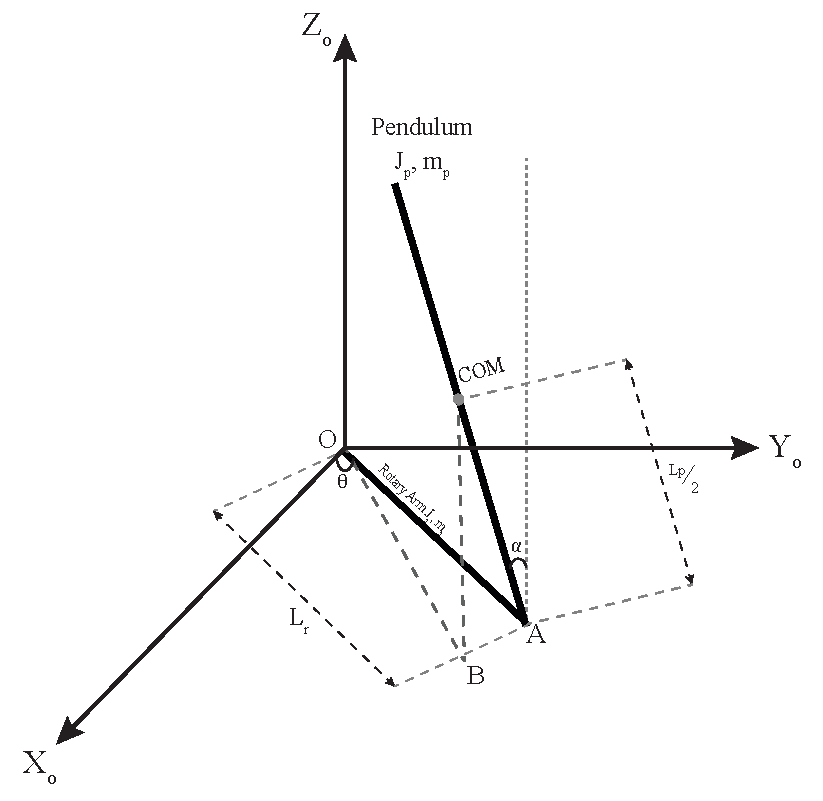
\includegraphics[width = \linewidth]{modelFigure.pdf}
            \caption{Schematic representation of the plant}
            \label{fig:modelFigure}
        \end{figure}
        %(add citation here)
        Although our system would not satisfy D'Alembert's principle of virtual work, i.e, the virtual displacements are orthogonal to constrain forces, due to the presence of non-conservative forces, these non-conservative forces can be augmented to the system without affecting the Lagrangian.

        The generalized coordinates for the system are the angular displacement of the rotating arm \(\theta\) and the pendulum angle \(\alpha\). The Lagrangian for a system is defined by (without non-conservative forces)
        \begin{equation}
            L = T - V
        \end{equation}
        where \(T\) is the kinetic energy and \(V\) is the potential energy of the system. \(\textbf{Note}\) that the dot convention for time derivative will be used throughout this document, i.e., \(\dot \theta = d\theta/d t\). Also \(t\) will be dropped from \(\theta\) and \(\alpha\). The kinetic energy of rotary arm is defined by the rotational kinetic energy 
        \begin{equation}
            T_{arm} = \frac{1}{2} J_r \dot \theta^2
        \end{equation}
        where \(J_r\) the moment of inertia of rotary arm at \(O\). The kinetic energy of the pendulum arm is the sum rotational kinetic energy and translational kinetic energy 
        \begin{equation}
            T_{pend} = \frac{1}{2} J_p \dot \alpha^2 + \frac{1}{2} m_p |\mathbf{\dot r_p}|^2 
        \end{equation}
        where \(J_p\) is the moment of inertia of pendulum arm at center of mass (COM), and \(\mathbf{r_p}\) is the position vector of COM of pendulum arm. Using cylindrical coordinates, the COM of pendulum arm is 
        \begin{equation}
            \mathbf{r_p} = \begin{bmatrix}
                \sqrt{L_r^2 + \frac{L_p^2}{4} s_\alpha^2} \\
                \theta - \tan^{-1}\left(\frac{L_p s_\alpha}{2 L_r}\right) \\
                \frac{L_p}{2} c_\alpha
            \end{bmatrix}_{(r,\psi,z)}
        \end{equation}
        where \(c_\psi = \cos \psi\) and \(s_\psi = \sin \psi\). The coordinate values of radial and angular position are calculated by looking at \(\triangle ABO\). The velocity is given by
        \begin{equation}
            |\mathbf{\dot r_p}|^2 = \dot r^2 + r^2 \dot \psi^2 + \dot z^2.
        \end{equation}
        Substituting and making some cancellations give
        \begin{equation}
            |\mathbf{\dot r_p}|^2 =\frac{1}{2} L_p^2 \dot \alpha^2 - L_p L_r c_\alpha \dot \alpha \dot \theta + \left(L_r^2 + \frac{1}{4} L_p^2 s_\alpha^2 \right) \dot \theta^2.
        \end{equation}
        The above equation incorporates the constrains of our system. The energy of conservative forces can be written as 
        \begin{gather}
            T = \frac{1}{2} J_r \dot \theta^2 + \frac{1}{2} J_p \dot \alpha^2 + \frac{1}{2} m_p |\mathbf{\dot r_p}|^2, \\
            V = \frac{1}{2} L_p c_\alpha .
        \end{gather}
        Euler-Lagrange equations for the system are of the form 
        \begin{gather}
            \dfrac{d}{dt}\left(\frac{\partial L}{\partial \dot \theta}\right) - \frac{\partial L}{\partial \theta} = Q_1 \\
            \dfrac{d}{dt}\left(\frac{\partial L}{\partial \dot \alpha}\right) - \frac{\partial L}{\partial \alpha} = Q_2
        \end{gather}
        where the generalized \(Q_i\) forces describe the non-conservative forces applied to the system with respect to the generalized coordinates. For our system, the generalized force acting on the rotary arm is 
        \begin{equation}
            Q_1 = \tau -B_r \dot \theta
        \end{equation}
        and acting on the pendulum is 
        \begin{equation}
            Q_2 = -B_p \dot \alpha
        \end{equation}
        where \(\tau\) is the torque acting on the rotary arm, and \(B_r,B_p\) are viscous damping force. The control variable is the input servo motor voltage \(V_m\) \((u(t))\) , and the torque generated by the servo motor is described by the equation \cite{gurocak_rotary_2017}
        \begin{equation}
            \tau = \frac{\eta K_g k_t(V_m - K_g k_m \dot \theta)}{R_m}
        \end{equation}

        Using \(q = [\theta,\alpha]^T\) the terms of Lagrangian equations can be written as 
        \begin{widetext}
            \begin{gather}
                \frac{\partial L}{\partial \dot q} = \begin{bmatrix}
                    \left(J_r + m_p L_r^2 + \frac{1}{4}m_p L_p^2 s_\alpha^2 \right)\dot \theta -\frac{1}{2} m_p L_r L_p c_\alpha \dot \alpha \\
                    \left(J_p +\frac{1}{4}m_p L_p^2\right) \dot \alpha - \frac{1}{2} m_p L_r L_p c_\alpha \dot \theta
                \end{bmatrix}, \\
                \frac{d}{dt}\left(\frac{\partial L}{\partial \dot q}\right) = 
                \begin{bmatrix}
                    \left(J_r + m_p L_r^2 +\frac{1}{4}m_p L_p^2 s_\alpha^2\right) \ddot\theta +\frac{1}{2}m_p L_p^2 c_\alpha s_\alpha \dot \alpha \dot \theta - \frac{1}{2} m_p L_r L_p c_\alpha \ddot \alpha + \frac{1}{2} m_p L_r L_p s_\alpha \dot \alpha^2 \\
                    \left(J_p +\frac{1}{4}m_p L_p^2\right) \ddot \alpha + \frac{1}{2} m_p L_r L_p s_\alpha \dot \alpha \dot \theta -\frac{1}{2} m_p L_r L_p c_\alpha \ddot \theta
                \end{bmatrix},\\
                \frac{\partial L}{\partial q} = \begin{bmatrix}
                    0 \\
                    \frac{1}{2} m_p L_p g s_\alpha + \frac{1}{2} m_p L_r L_p s_\alpha \dot \alpha \dot \theta + \frac{1}{4} m_p L_p^2 c_\alpha s_\alpha \dot \theta^2  
                \end{bmatrix}.
            \end{gather}
        \end{widetext}
        Finally, equations (13)-(16) can be rearranged into manipulator equation form 
        \begin{equation}
            H(q) \ddot q + C(q,\dot q) \dot q + G(q) = Bu, \label{eq:manipulatorEq}
        \end{equation}
        where, 
        \begin{gather*}
            H(q) = \begin{bmatrix}
                J_r +\frac{1}{4}m_p L_p^2 s_\alpha^2 + m_p L_r^2 & -\frac{1}{2} m_p L_p L_r c_\alpha\\
                -\frac{1}{2} m_p L_p L_r c_\alpha & J_p +\frac{1}{4} m_p L_p^2
            \end{bmatrix} \\
            C(q,\dot q) = \begin{bmatrix}
                \frac{1}{4} m_p L_p^2 s_{2\alpha} \dot \alpha + \frac{\eta K_g^2 k_t k_m}{R_m} + B_r & \frac{1}{2} m_p L_r L_p s_\alpha \\
                -\frac{1}{8}m_p L_p^2 s_{2\alpha} \dot \theta & B_p
            \end{bmatrix} \\
            G(q) = \begin{bmatrix}
                0\\
                -\frac{1}{2} m_p L_p g s_\alpha 
            \end{bmatrix}\\
            B = \begin{bmatrix}
                \frac{\eta K_g K_t }{R_m} \\
                0
            \end{bmatrix}
        \end{gather*}
        Note, that the choice of \(C(q,\dot q)\) is not unique. The manipulator Equation (\ref{eq:manipulatorEq}) can be rearranged to solve for \(\ddot q\)
        \begin{equation}
            \ddot q = \begin{bmatrix}
                \ddot \theta\\
                \ddot \alpha
            \end{bmatrix}
             = H(q)^{-1}\left(Bu - C(q,\dot q) \dot q -G(q)\right)
        \end{equation}
        Using the above equation, the full non-linear system can be written out as 
        \begin{align}
            \dot \bx = f(\bx,u) \label{eq:nonLinearSystem}
        \end{align} 
        where \(\bx = [q,\dot q]^T\), and 
        \begin{equation}
            f(\bx,u) = \begin{bmatrix}
                \dot q \\
                H(q)^{-1}\left(Bu - C(q,\dot q) \dot q -G(q)\right)
            \end{bmatrix} \nonumber
        \end{equation}
        The full-nonlinear plant is simulated in MATLAB by integrating the above equation. The plant schematic is shown in Fig. ref. 
    }
    \section{System Linearization}{
        The linearized dynamics of any system \(\dot x = f(x,u)\) around a equilibrium point (fixed point) \((x^*,u^*)\) can be determined by Taylor expansion 
        \begin{equation*}
            \dot x \approx f(x^*,u^*) + \left.\frac{\partial f}{\partial x}\right|_{x^*,u^*} (x - x^*) + \left.\frac{\partial f}{\partial u}\right|_{x^*,u^*} (u - u^*)
        \end{equation*}
        therefore at fixed point 
        \begin{equation*}
            \dot x \approx  \left.\frac{\partial f}{\partial x}\right|_{x^*,u^*} (x - x^*) + \left.\frac{\partial f}{\partial u}\right|_{x^*,u^*} (u - u^*).
        \end{equation*}
        Although in this example we used scalar functions \(f,x,u\) the same series expansion can be used to vector valued functions where the partial derivatives are replaced with their vector equivalent Jacobian matrices (\(\nabla_{\mathbf{x}} \mathbf{f}\), \(\nabla_{\mathbf{u}} \mathbf{f}\)). 
        
        Even through this method of linearization can be performed for system represented in Eq.\ref{eq:nonLinearSystem}, we won't be proceeding with this as the calculations are quite cumbersome. The tidiest way to make an approximation near an equilibrium point is to introduce new variables which are small.  Thus we can write \(\theta = \theta_{eq} + \theta_\epsilon\), \(\alpha = \alpha_{eq} +\alpha_\epsilon\) and \(u = u_{eq}\) where \(\tee\) and \(\aee\) are considered to be small. The equilibrium point of the system are calculated by setting all time derivatives of Eq.\ref{eq:manipulatorEq} to \(0\), i.e., \(\dot{q} \to 0, \ddot q \to 0\). This gives 
        \begin{gather}
            G(q) = B u_{eq} \Rightarrow u_{eq} = 0, \alpha = 0,\pi \nonumber
        \end{gather}
        The equilibrium points of the system are
        \begin{align*}
            (\theta_{eq},0) && (\theta_{eq},\pi)
        \end{align*}
        where \(\theta_{eq} \in \R\). As expected, this system has a moving equilibrium which is independent of \(\theta\). We are interested in the dynamics of the inverted pendulum state \(\alpha_{eq} = 0\). Substituting these new variables into the original ODE and keeping only linear terms gives 
        \begin{gather}
            H = \begin{bmatrix}
                J_r + m_p L_r^2 & -\frac{1}{2} m_p L_p L_r\\
                -\frac{1}{2} m_p L_p L_r & J_p +\frac{1}{4} m_p L_p^2
            \end{bmatrix}\\
            C = \begin{bmatrix}
                \frac{\eta K_g^2 k_t k_m}{R_m} + B_r & 0 \\
                0 & B_p
            \end{bmatrix}\\
            G = \begin{bmatrix}
                0\\
                -\frac{1}{2} m_p L_p g \aee 
            \end{bmatrix}
        \end{gather}
        Here the approximation \(\sin\aee \approx \aee\) and \(\cos\aee \approx 1\) was used to simplify the equations. Solving for acceleration terms, we get 
        \begin{gather}
            \left[\begin{array}{l}
                \ddot{\tee} \\
                \ddot{\aee}
                \end{array}\right]=H^{-1}\left[\begin{array}{c}
                \frac{\eta K_g k_t(u - K_g k_m \dot \tee)}{R_m}-B_{r} \dot{\tee} \\
                \frac{1}{2} m_{p} L_{p} g \aee-B_{p} \dot{\aee}
                \end{array}\right].
        \end{gather}
        The above equations are linear (H is a constant matrix) and therefore can be represented in state space form. Moving back to original variables \((\theta,\alpha)\) and expanding the above matrix gives 
        \begin{widetext}
            \begin{gather}
                \ddot \theta = \frac{1}{\Delta} \left(-\left(J_{p}+\frac{1}{4} m_{p} L_{p}^{2}\right)\left(\frac{\eta K_g^2 k_t k_m}{R_m}+B_{r}\right)  \dot{\theta}-\frac{1}{2} m_{p} L_{p} L_{r} B_{p} \dot{\alpha}+\frac{1}{4} m_{p}^{2} L_{p}^{2} L_{r} g \alpha+\left(J_{p}+\frac{1}{4} m_{p} L_{p}^{2}\right) \frac{\eta K_g k_t u}{R_m}\right) \\
                \ddot{\alpha}=\frac{1}{\Delta}\left(-\frac{1}{2} m_{p} L_{p} L_{r} \left(\frac{\eta K_g^2 k_t k_m}{R_m}+B_{r}\right) \dot{\theta}-\left(J_{r}+m_{p} L_{r}^{2}\right) B_{p} \dot{\alpha}+\frac{1}{2} m_{p} L_{p} g\left(J_{r}+m_{p} L_{r}^{2}\right) \alpha+\frac{1}{2} m_{p} L_{p} L_{r} \frac{\eta K_g k_t u}{R_m}\right) \\
                A = \frac{1}{\Delta}\begin{bmatrix}
                    0 & 0 & 1 & 0 \\
                    0 & 0 & 0 & 1 \\
                    0 & \frac{1}{4} m_{p}^{2} L_{p}^{2} L_{r} g & -\left(J_{p}+\frac{1}{4} m_{p} L_{p}^{2}\right)\left(\frac{\eta K_{g}^{2} k_{t} k_{m}}{R_{m}}+B_{r}\right) & -\frac{1}{2} m_{p} L_{p} L_{r} B_{p} \\
                    0 & \frac{1}{2} m_{p} L_{p} g\left(J_{r}+m_{p} L_{r}^{2}\right) & -\frac{1}{2} m_{p} L_{p} L_{r}\left(\frac{\eta K_{g}^{2} k_{t} k_{m}}{R_{m}}+B_{r}\right) & -\left(J_{r}+m_{p} L_{r}^{2}\right) B_{p}
                \end{bmatrix} \\
                B = \frac{\eta K_g k_t}{\Delta R_m}
                \begin{bmatrix}
                    0\\
                    0\\
                    J_{p}+\frac{1}{4} m_{p} L_{p}^{2}\\
                    \frac{1}{2} m_{p} L_{p} L_{r}
                \end{bmatrix}
            \end{gather}
        \end{widetext}
        where \(\Delta = \det(H)\). After collecting the terms and arranging, we get the above state space matrices. Some of the computations above were preformed using \textit{Mathematica} as it was too cumbersome and error prone to be performed by hand. After substituting parameter values from Table. \ref{tab:systemData}, the state space matrices are 
        \begin{align*}
            A = \begin{bmatrix}
                0 & 0 & 1 & 0\\
                0 & 0 & 0 & 1 \\
                0 & 12.27 & -8.67 &-0.0764\\
                0 & 51.44 &-3.49 &-0.32
            \end{bmatrix} &&
            B = \begin{bmatrix}
                0\\
                0\\
                15.07\\
                6.0715
            \end{bmatrix} \\
            C = \begin{bmatrix}
                1 & 0 & 0 & 0\\
                0 & 0 & 0 & 0
            \end{bmatrix} &&
            D = \begin{bmatrix}
                0 \\ 
                0
            \end{bmatrix}
        \end{align*}
        By computing the reachability matrix, we see that the system is controllable. Also, we see that the system is unstable as \(A\) has positive eigenvalues. We also see that the system is observable as the observability matrix is full rank. To see how well the linearized system performs, the linear and non linear system with step impulse is plotted in Fig.\ref{fig:LinearNonLinear}
        \begin{figure}[h!]
            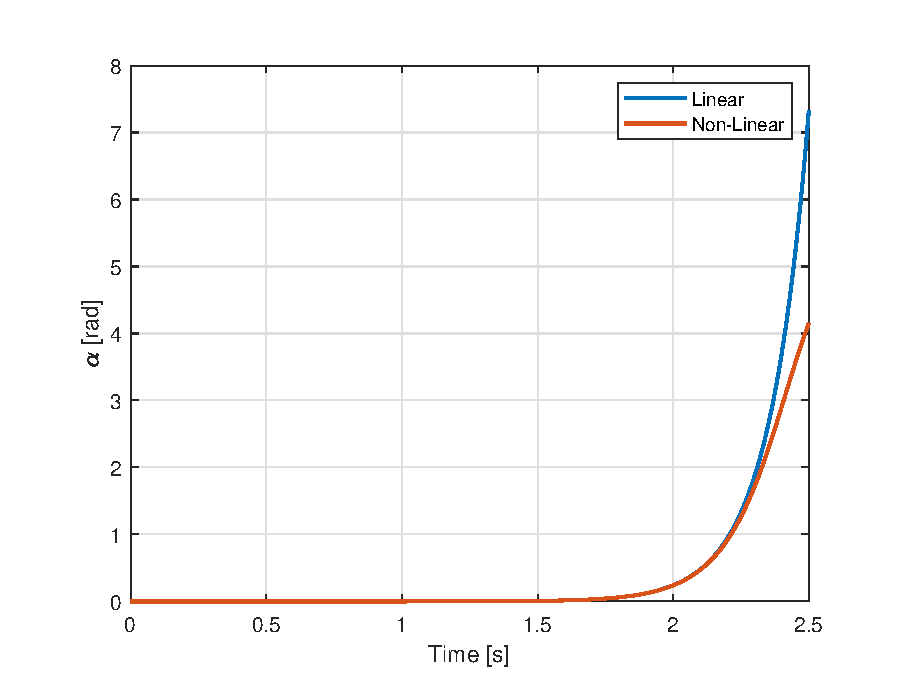
\includegraphics[width = \linewidth]{LinearNonLinear.eps}
            \caption{Comparison of Linear and Non-Linear system}
            \label{fig:LinearNonLinear}
        \end{figure}
    }
    \section{Controller Design and Simulations}
    {
        In this section, we will be discussing and designing these components
        \begin{itemize}
            \item A full state feedback controller for stabilizing inverted position 
            \item A state observer to estimate state and attenuate signal noise
            \item A Swing up controller 
            \item A Non-Linear observer to observe the full state of the system
        \end{itemize}
        \subsection{Full state feedback controller}{
            The requirements of full state feedback controller are:
            \begin{enumerate}
                \item Smoothly and precisely achieve any rotary angle \(\theta\)
                \item Maintain stability in the presence of noisy signals
            \end{enumerate}
            The primary considerations for this system is to determine the expected system characteristics like,overshoot, rise time, and settling time. As this system is quite unstable and can enter non-linear region quite easily, the controller must have low overshoot with a sufficiently large rise time and settling time. Rapid changes in angles or controller effort can push the system to non-linear region and would result the pendulum falling off. 

            The maximum overshoot for the system was determined to be 5\%. Having a low overshoot will reduce the overall controller effort and provide a smooth transition from one reference point to another. The settling time is an important factor for stability. A quick stabilization time of < 2 would provide quick response as well as a fast stabilization. Finally, we also require that the pendulum angle \(|\alpha| < 15^\circ\) and the controller effort is less than the maximum voltage \(|V_m| < 6\)V.
        }
        
        With the required characteristics of the system outlined, we can calculated the desired pole locations. The percentage of overshoot is calculated by 
        \begin{equation}
            M_p = e^{-\zeta \pi / \sqrt{1-\zeta^{2}}}
        \end{equation}
        where \(\zeta\) is the damping constant of the system. A 5\% overshoot corresponds to 
        \begin{equation}
            \zeta = \frac{1}{\sqrt{2}} \approx 0.7 
        \end{equation}
        With a settling time \(T_s = 2\) seconds, the natural frequency of the system can be approximated 
        \begin{equation}
            T_s = \frac{4}{\zeta \omega_n} \Rightarrow \omega_n = 2.857 \text{rad/s}
        \end{equation}
        From this, the desired dominant poles are 
        \begin{equation}
            p_{1,2}=-\sigma \pm j \omega_{d}
        \end{equation}
        where \(\sigma = \zeta \omega_n\) and \(\omega_d = \omega_n \sqrt{1-\zeta^2}\). Substituting the above values,we get the following two dominant poles 
        \begin{equation}
            p_{1,2} = -2 \pm 2.04 j
        \end{equation}
        The non dominant poles of this system are set far from the desired poles so that they have no significant impact on the system response. The non-dominant poles were set to \(p_{3,4}=-30,-40\). The controller gains can be easily calculated using MATLAB `place' functions which will calculate the required gains so \(A-BK\) have the desired eigenvalues. These poles are placed by optimizing the choice of eigenvectors for a robust solution \cite{kautsky_robust_1985}. The controller gains are 
        \begin{equation}
            K = \begin{bmatrix}
                -13.97 & 293.83 &  -8.32 &  31.38
            \end{bmatrix}
        \end{equation}
        Finally, the closed loop response of the non-linear plant with the controller is shown in Fig.\ref{fig:closedControl}. In this simulation, a reference generator is used which change \(\theta = [30,-60,45,-30]^\circ\) once it has stabilized (threshold of \(3^\circ\)) at a position for more than 3 seconds. The step output from the reference generator is passed through a \(1^{st}\) order low pass filter to smooth out the signal. 
        \begin{figure}[t!]
            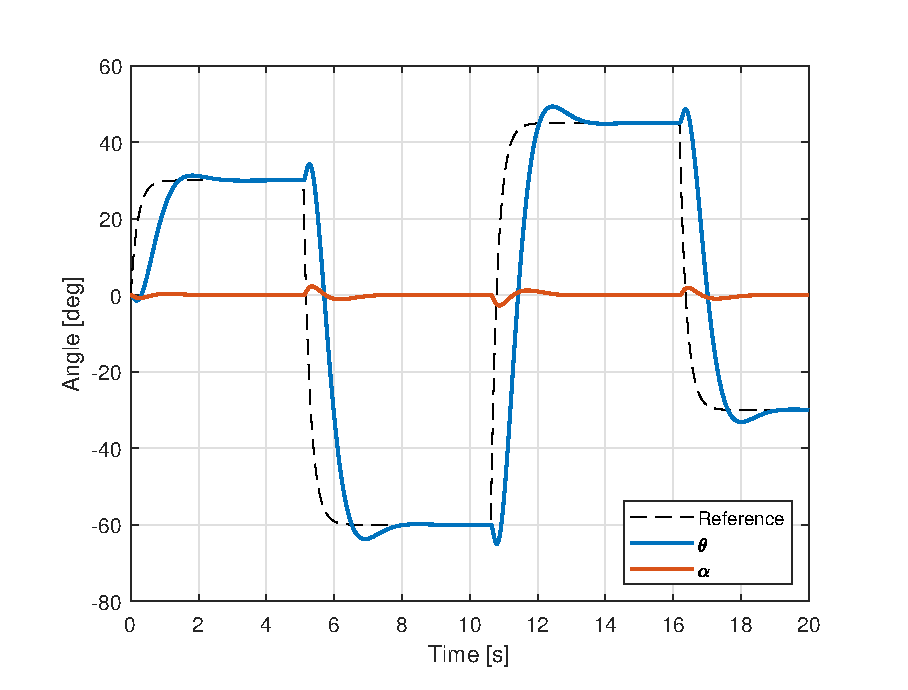
\includegraphics[width = \linewidth]{closedControl.eps}
            \caption{Closed loop response of the Non-linear plant}
            \label{fig:closedControl}
        \end{figure}
        \begin{figure}[t!]
            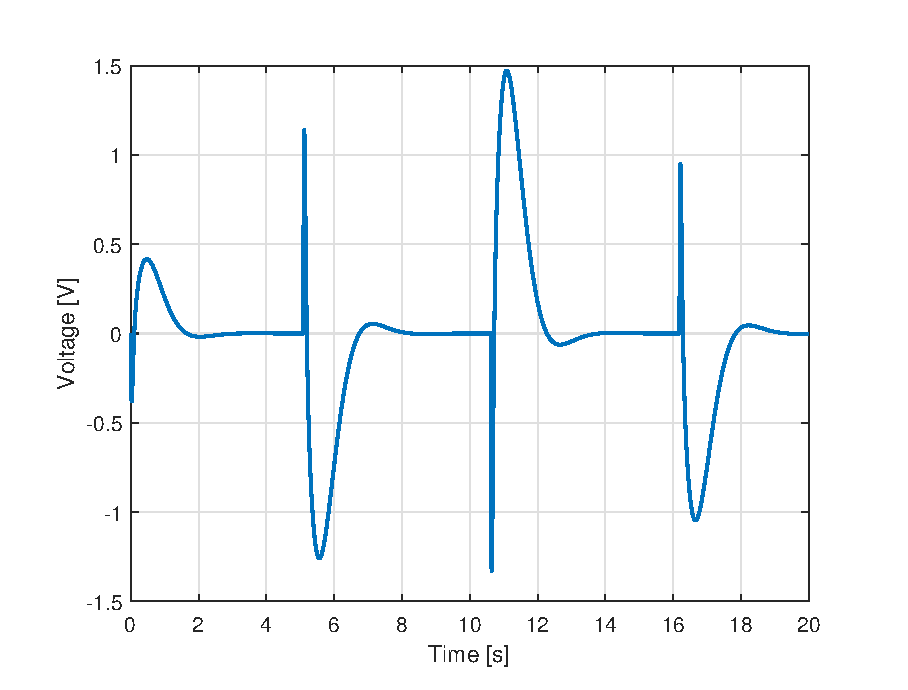
\includegraphics[width = \linewidth]{controllerEffort.eps}
            \caption{Closed loop controller output}
            \label{fig:controllerEffort}
        \end{figure}
        The controller effort during this simulation is well below the threshold and is shown in Fig. \ref{fig:controllerEffort}. The system is also able to maintain the pendulum upright when there a signal noise of \(10^{-2}\) order. This was tested by adding white noise to the output signal and is shown in Fig.\ref{fig:withNoise}. 
        \begin{figure}[t!]
            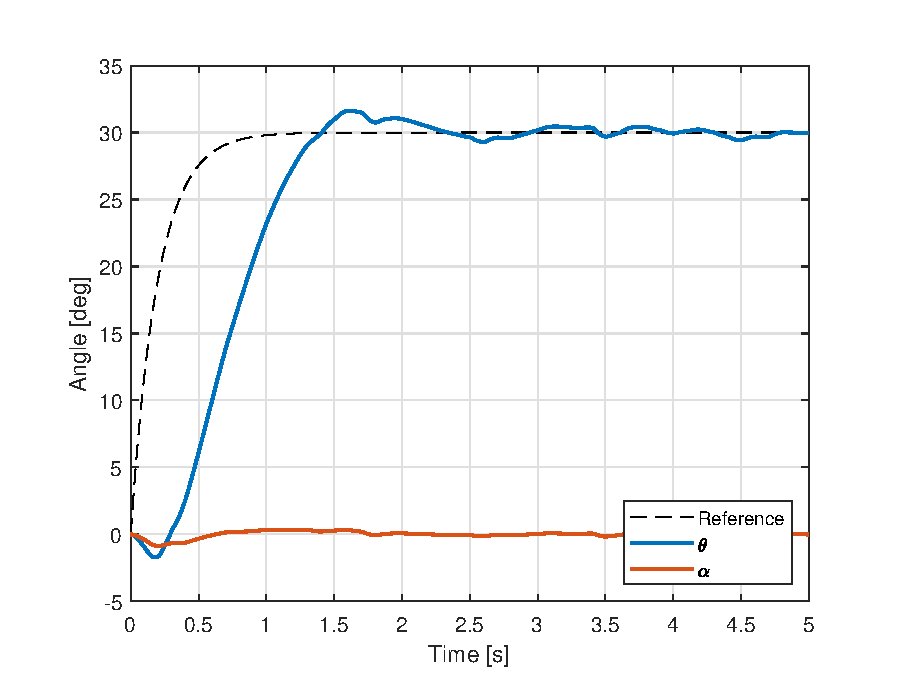
\includegraphics[width = \linewidth]{withNoise.eps}
            \caption{Closed loop response with white noise of order \(10^{-2}\) added to output signal}
            \label{fig:withNoise}
        \end{figure}
        \subsection{Designing a Linear state estimator}{
            As our system does not have dedicated sensors to measure the angular velocity of the pendulum or the arm, we need to estimate these states with knowledge of current position and controller input. One novel but an inefficient solution would be time derivate of position to get angular velocity. Even though in an idealized situation, this would be feasible, but most sensor outputs have noise. Therefore, a linear state estimator with noise attenuation is required.   

            A general linear observer have a form 
            \begin{equation}
                \frac{d \hat x}{dt} = A\hat x + Bu + L(y - C\hat x)
            \end{equation}
            where \(L\) is the observer gains and \(\hat x\) is the estimated state. The estimated error \(\tilde{x}=x-\hat{x}\) would have the dynamics 
            \begin{equation}
                \frac{d \tilde{x}}{d t}=(A-L C) \tilde{x}.
            \end{equation}
            Then by choosing \(L\) such that \(A - LC\) have eigenvalues with negative real parts will ensure that the error will converge to \(0\). The convergence rate is determined by the appropriate selection of \(L\). Choosing large negative eigenvalues will allow the observe to converge quickly, but will also be sensitive to noise. Therefore, the gains are selected such that estimator converges about twice as fast as the dynamics of the closed loop system. This allows a good estimate of the current state at the same time being insensitive to signal noise. 

            With the above fact taken into considerations, the closed loop poles of the observer are selected beyond \(\Re(p) = -4\). The selected poles are 
            \begin{equation}
                p = \begin{bmatrix}
                    -4 & -4.5 & -5 & -5.5 
                \end{bmatrix}.
            \end{equation}
            Using the poles, calculated observer gains are 
            \begin{equation}
                L  = \begin{bmatrix}
                    1.37  &-0.134 \\
                    -2.72 &   8.64\\
                    13.26  & 12.51\\
                    -0.296  & 68.95
                \end{bmatrix}.
            \end{equation}
            Using this observer, we can use the same controller designed in the previous section as a consequence of separation principle. This allows up to independently assign eigenvalues for a controller and observer and combine them together. The full Simulink system is shown in Fig. \ref{fig:linearSysWithO}. 
            \begin{figure}
                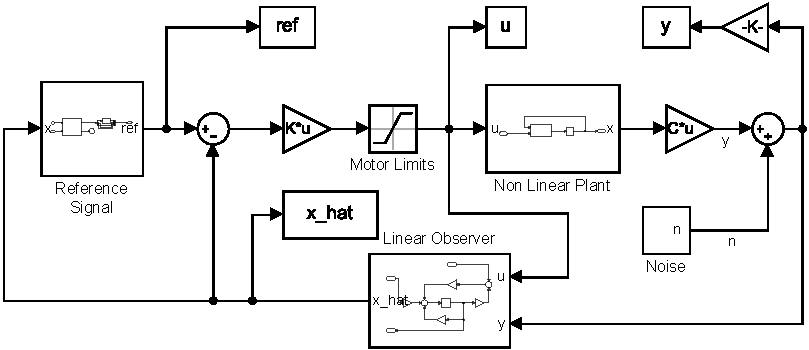
\includegraphics[width = \linewidth]{linearSysWithO.pdf}
                \caption{Closed loop controller output}
                \label{fig:linearSysWithO}
            \end{figure}
            Even with large signal noise added to the system, the observer is able to estimate the states accurately which allows controller to move the pendulum accurately. The output signal \(y\) and the estimated value is shown in Fig. \ref{fig:EstimateState}. As we can see, the system is still being able to maintain the pendulum vertical and track quite accurately. The system does spend more time at \(\theta = 45^\circ\) because it fails to maintain a stable angle with a threshold of \(3^\circ\) for more than 3 seconds. Finally, the controller output is checked and it is also well below the \(6\) V threshold.   
            \begin{figure}
                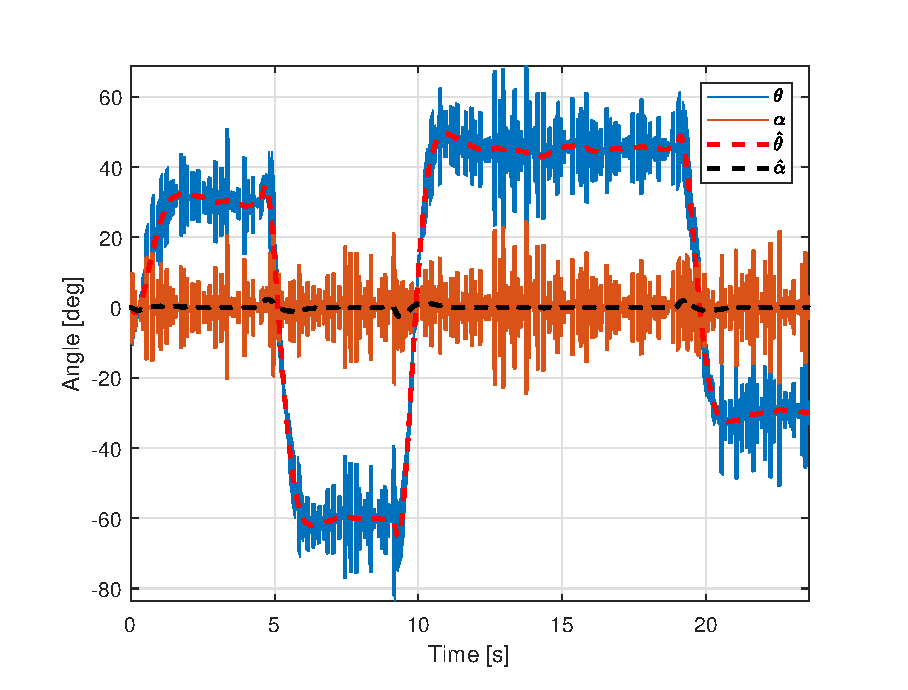
\includegraphics[width = \linewidth]{EstimateState.eps}
                \caption{Comparison between output signal \(y\) and estimated state \(\hat x\). Here signal noise }
                \label{fig:EstimateState}
            \end{figure}
        }
        \subsection{Swing up control}{
            The objective of this controller is to bring the pendulum from downward position to vertically upright position, then the full state feedback controller can stabilize the pendulum at this state. A switching logic is used to switch over from swing up control to stabilization control. 

            The swing up action is attained using an energy controller. Here the total energy of the system is used as a feedback quantity \cite{astrom_swinging_1996} \cite{akhtaruzzaman_modeling_2010}. It is driven such a way that the system achieves the energy equal to the upright position. By neglecting frictional losses, we can write refine the dynamics of the pendulum in terms of pivot acceleration as 
            \begin{equation}
                J_{p} \ddot{\alpha} = \frac{1}{2} m_{p} L_{p} u \cos \alpha + \frac{1}{2} m_{p}  L_{p} g\sin \alpha
            \end{equation}
            where \(u\) is the pivot acceleration. The energy of the pendulum in pivot frame is 
            \begin{equation}
                E=\frac{1}{2} J_{p} \dot{\alpha}^{2}+\frac{1}{2} m_{p} g L_{p}\cos \alpha.
            \end{equation}
            Taking time derivative of the above equation and simplifying gives 
            \begin{equation}
                \dot{E}= \frac{1}{2} m_{p} L_{p} u \dot{\alpha} \cos \alpha
            \end{equation}
            From the above equation, we can see that the energy of the pendulum is simply an integrator with varying gains. A control strategy where 
            \begin{equation}
                u=\left(E-E_{r}\right) \dot{\alpha} \cos \alpha
            \end{equation}
            would drive the system to the desired energy \(E_r\). The above control law is non-linear and depends on pendulum angle \(\alpha\) and \(\dot \alpha\). From Eq. 39, we can see that required reference energy for the pendulum to be upright is \(1/2 \ m_p L_p g\)J. 

            As the system has damping forces, it is necessary to change the energy quickly. We can modify the control law to 
            \begin{equation}
                u = \operatorname{sat}_{u_{\max }}\left(\mu\left(E-E_{r}\right) \operatorname{sign}(\dot{\alpha} \cos \alpha)\right) \label{eq:uControlEq}
            \end{equation}
            where \(\mu\) is a controller gain, \(\operatorname{sat}_{u_{\max }}\) function saturates the control signal's maximum acceleration. This controller basically acts like a bang-bang controller for large errors and as a proportional control for small errors.

            Finally, the pivot acceleration is transformed into servomotor voltage to get 
            \begin{equation}
                V_{m}=\frac{R_{m} J_r u}{\eta_{g} K_{g} \eta_{m} L_r k_{t}}+K_{g} k_{m} \dot{\theta}
            \end{equation}
            where \(\tau = J_r / L_r\). 
            
            The energy control subsystem is shown in Fig. \ref{fig:EnergyController}. This subsystem encapsulates Eq.\ref{eq:uControlEq}. The controller output voltage is calculated by the Swing up controller shown in \ref{fig:SwingUp}. 
            \begin{figure}
                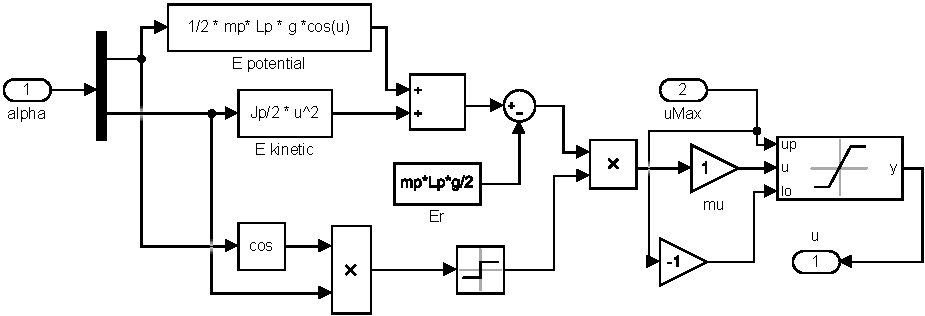
\includegraphics[width = \linewidth]{EnergyControl.pdf}
                \caption{Energy controller subsystem. This subsystem takes \(\alpha, \dot \alpha\) and calculates the required pivot velocity \(u\)}
                \label{fig:EnergyController}
            \end{figure}
            \begin{figure}
                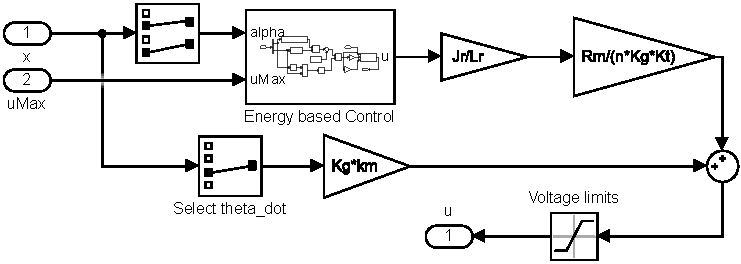
\includegraphics[width = \linewidth]{SwingUp.pdf}
                \caption{Swing Up Controller. This system takes \(\bx\) and calculates the controller output voltage}
                \label{fig:SwingUp}
            \end{figure}
            \begin{figure}
                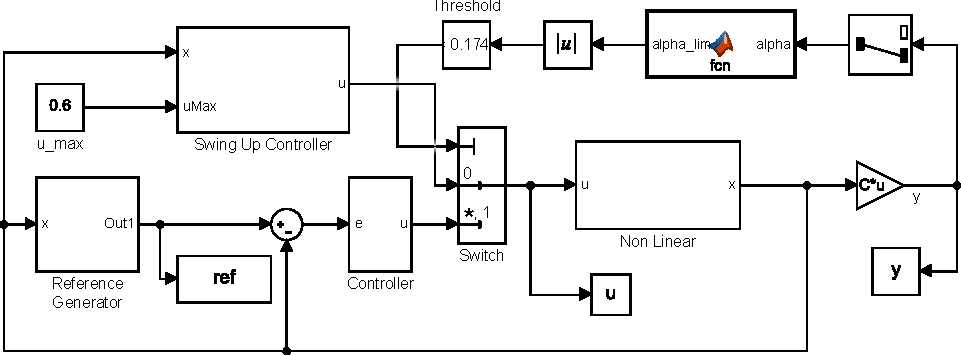
\includegraphics[width = \linewidth]{SwingUpSystem.pdf}
                \caption{Swing up system}
                \label{fig:SwingUpSystem}
            \end{figure}
            
            To combine the swing up controller with the feedback controller, a switching logic is used which switches control over to the feedback controller when the pendulum is vertical. A function block is used that converts \(\alpha \in (-\pi,\pi)\) so that the switch and controller works as expected. The switch logic can be summarized as 
            \begin{equation}
                u = \begin{cases}
                    K(\mathbf{r} - \bx) & |\alpha| < 10^\circ \\
                    \operatorname{sat}_{u_{\max }}\left(\mu\left(E-E_{r}\right) \operatorname{sign}(\dot{\alpha} \cos \alpha)\right) & \text{Otherwise}.
                \end{cases}
            \end{equation}
            The combined system is shown in Fig.\ref{fig:SwingUpSystem}.

            To see the controller in action, the pendulum was given a small oscillation in the downward position. This is necessary as \(\dot \alpha \cos \alpha\) would be zero, resulting in zero controller output. Once there is small oscillations, the pendulum starts swinging until it becomes vertical. The system in action is shown in Fig. \ref{fig:SwingUpAction}. Once the pendulum is vertical and stable, the reference generator moves the pendulum to different set points. 

            \begin{figure}
                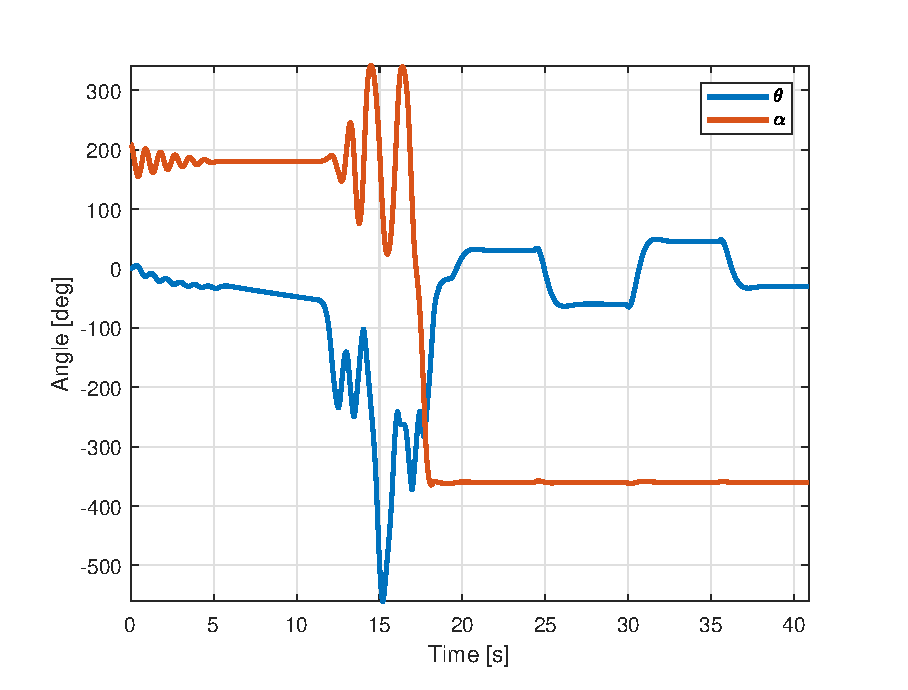
\includegraphics[width = \linewidth]{SwingUpAction.eps}
                \caption{Swing up action of the Pendulum}
                \label{fig:SwingUpAction}
            \end{figure}
            \begin{figure}
                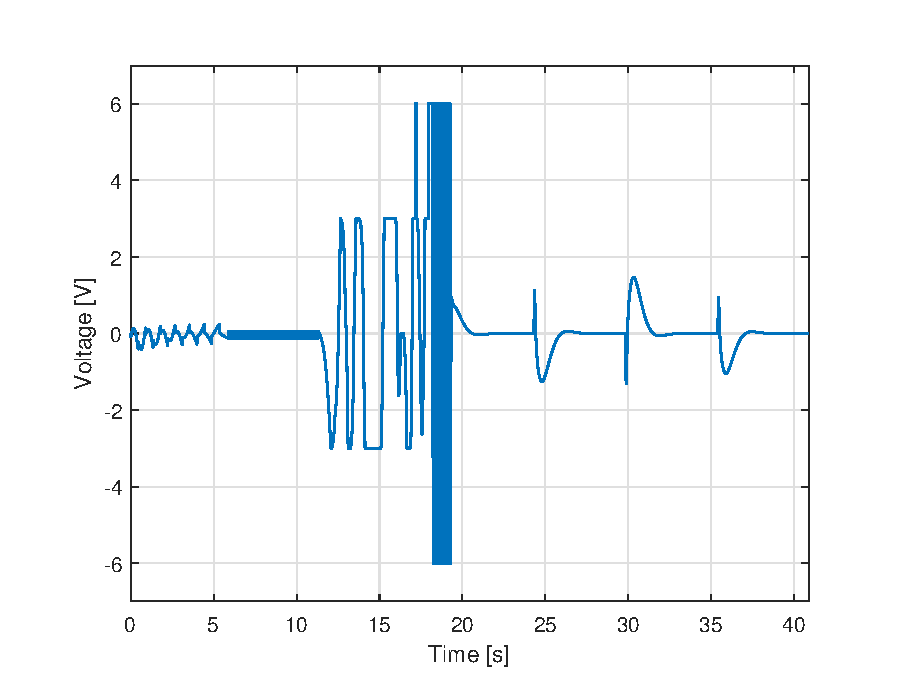
\includegraphics[width = \linewidth]{controllerEffortSwing.eps}
                \caption{Controller effort during swing up action}
                \label{fig:controllerEffortSwing}
            \end{figure}
            
            Although the controller makes the pendulum vertical, it doesn't perform it with minimum energy. The controller often exerts large effort which results in multiple pendulum windups. Also, the rotary arm moves large angles to swing up the pendulum. The controller effort is shown in Fig.\ref{fig:controllerEffortSwing}. As we can see, the controller effort saturates just after the swing up action. This unusual behavior is seen just after the swing up controller gives control to the feedback controller. Due to the large input, the pendulum swings over and control is regained after the second swing. This can be seen in \ref{fig:SwingUpAction} where the controller fails to maintain vertical position when \(\alpha = 0\). Changing the switch threshold angle did not fix this issue. 

        }
        \subsection{Designing a Non-Linear Observer}
        {
            During the swing up action or when the pendulum is down, the linear observer designed in the previous section cannot be used to estimate the full state of the system. This is because, the states are very far from the linearization point. To observe these states, a non-linear observer is proposed. The idea behind this is to design a time varying gain \(L(\hat \bx)\) such that  
            \begin{equation}
                \frac{d \hat x}{dt} = f(\hat \bx, u) + L(\hat \bx) (y - C \hat x)
            \end{equation}
            converges to the true state. Here, \(f(\bx,u)\) is the full non-linear system described in Eq. \ref{eq:nonLinearSystem}. 

            To calculate \(L(\hat \bx,t)\), the system is linearized at the estimated operating point
            \begin{equation}
                f(\hat \bx,u) \approx f\left(\hat \bx^*, u^*\right)+\nabla_{\mathbf{x}} \mathbf{f}_{x^{*}, u^{*}}\left(\hat \bx-\hat\bx^{*}\right)+\nabla_{\mathbf{u}} \mathbf{f}_{x^{*}, u^{*}}\left(u-u^{*}\right)
            \end{equation}
            where \(\hat \bx^*, u^*\) is the current estimated state and \(\hat \bx,u\) is the next estimated state. By using \(A :=\nabla_{\mathbf{x}} \mathbf{f}\) and \(B :=\nabla_{\mathbf{u}} \mathbf{f}\), the observer gain are calculated such that the eigenvalues of \(A - LC\) have negative real parts. This allows the observer converge to the true state of the system. 

            The analytical expression for \(A\) and \(B\) were calculated in \textit{Mathematica} and then imported as a matrix expression to Matlab. These expressions are too long to be expressed in this report. Using these matrices, the observer gains are calculated by using a modified `place' function. Some modifications were needed to the original `place' function to make it compatible for code generation. The same observer poles were that was used for linear observer was used to calculate \(L(\hat \bx)\). The schematic of the full-state observer is shown in Fig.\ref{fig:NonLinearObserver}

            \begin{figure}
                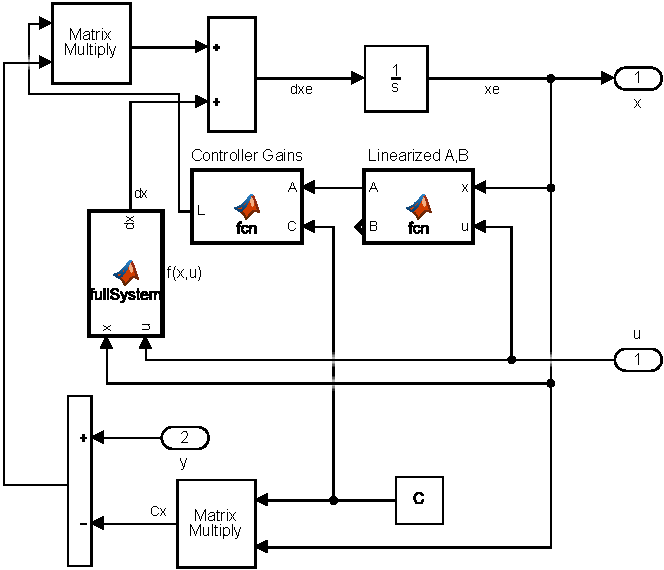
\includegraphics[width = 0.8\linewidth]{NonLinearObserver.pdf}
                \caption{Schematic representation of Non-Linear Observer.}
                \label{fig:NonLinearObserver}
            \end{figure}

            \begin{figure}
                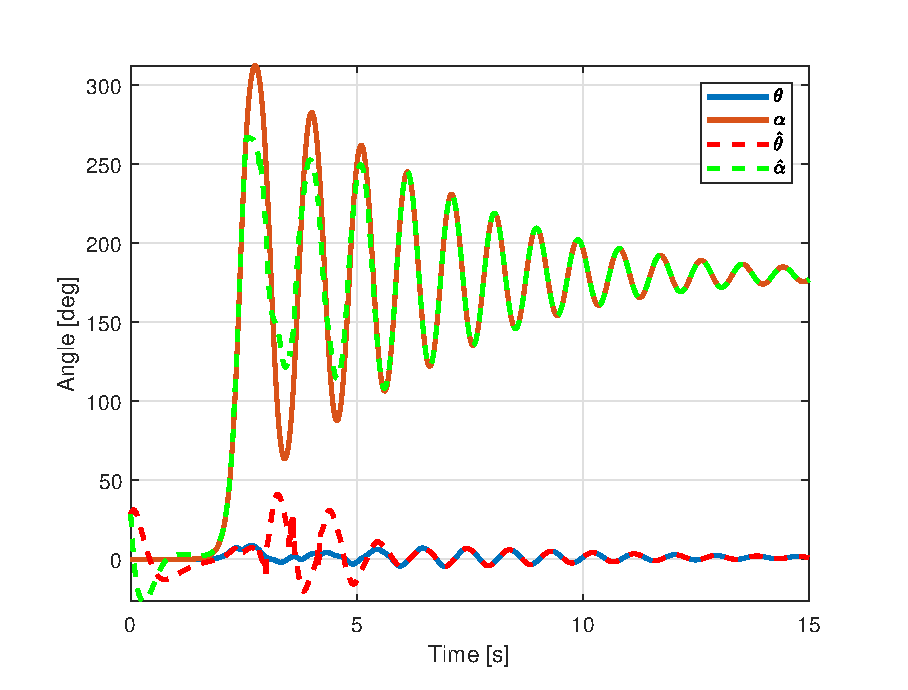
\includegraphics[width = \linewidth]{nonLinearOb.eps}
                \caption{Non Linear observer converging to state angular position when the pendulum falls down.}
                \label{fig:NonLinearOb}
            \end{figure}

            \begin{figure}
                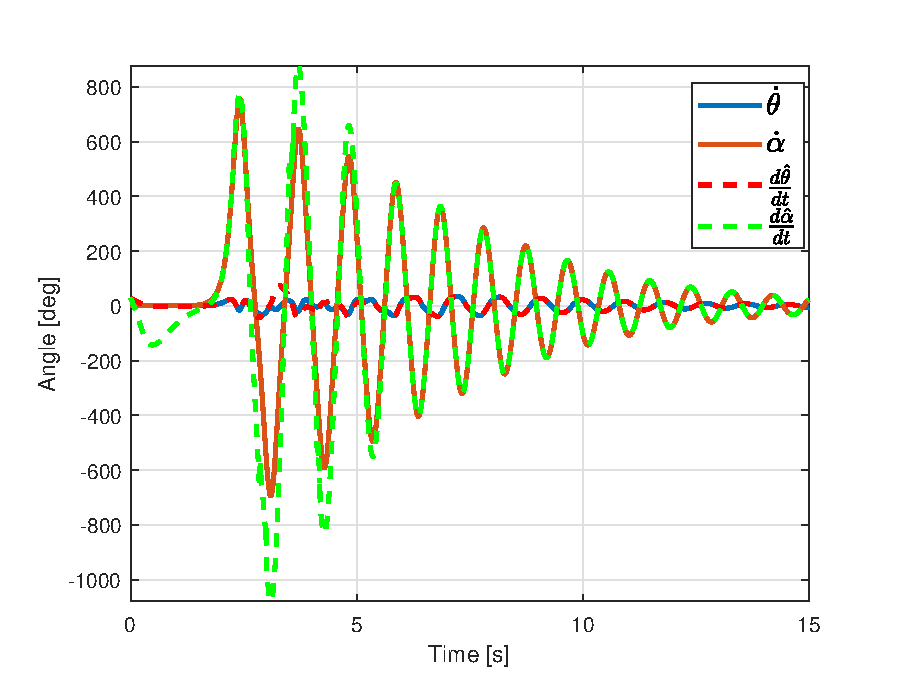
\includegraphics[width = \linewidth]{NonLinearObVel.eps}
                \caption{Non Linear observer converging to state angular velocity when the pendulum falls down.}
                \label{fig:NonLinearObVel}
            \end{figure}

            \begin{figure*}
                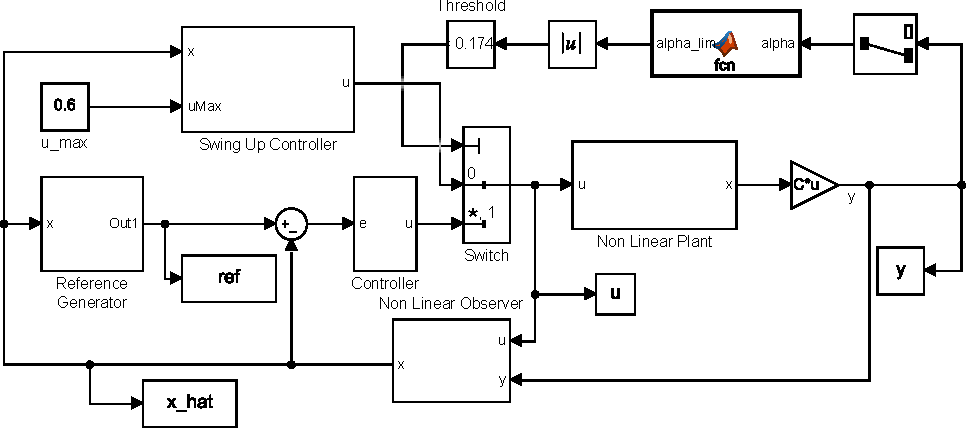
\includegraphics[width = \linewidth]{SwingUpSystemNonLin.pdf}
                \caption{Swing up system with non-linear observer}
                \label{fig:SwingUpSystemNonLin}
            \end{figure*}

            To test this observer, open loop response of the system and the observer were compared when the vertical pendulum was disturbed with a small impulse voltage. The observer was initialed at \(\bx = [0.5,0.5,0.5,0.5]^T\) to see the convergence of the estimated state and actual state. Fig.\ref{fig:NonLinearOb}, \ref{fig:NonLinearObVel} shows how the estimator converges to the true state. 

            Unfortunately, adding the non-linear observer to the swing up system causes convergence error which crashes the simulation. The automatically selected solver, ode15s crashes when the swing up controller outputs a large voltage. Using a different solver like ode45 did provides an output, but the swing up action was lost. This could be because of the non-linear nature of the swing up controller. The schematic represented of this system is shown in Fig.\ref{fig:SwingUpSystemNonLin}.

            Even though the swing up action failed when ode45 was used, the estimated state and actual state were compared to see the performance of the observer. The observer was initialized at \(\bx = [0.5,0.5,0.5,0.5]^T\) and the pendulum system at \(\bx = [0,\pi + 0.5,0,0]^T\) and the result is shown in Fig.\ref{fig:SwingupfailVel}, \ref{fig:swingFailPos}

            \begin{figure}
                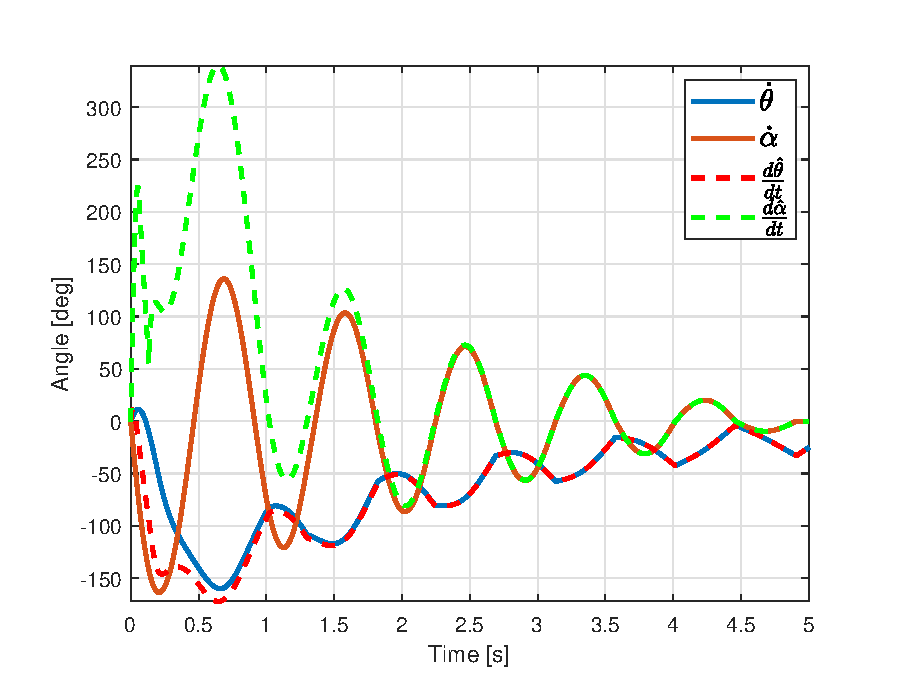
\includegraphics[width = \linewidth]{SwingupfailVel.eps}
                \caption{Non-linear estimator converging to true state angular velocity during a failed swing up.}
                \label{fig:SwingupfailVel}
            \end{figure}

            \begin{figure}
                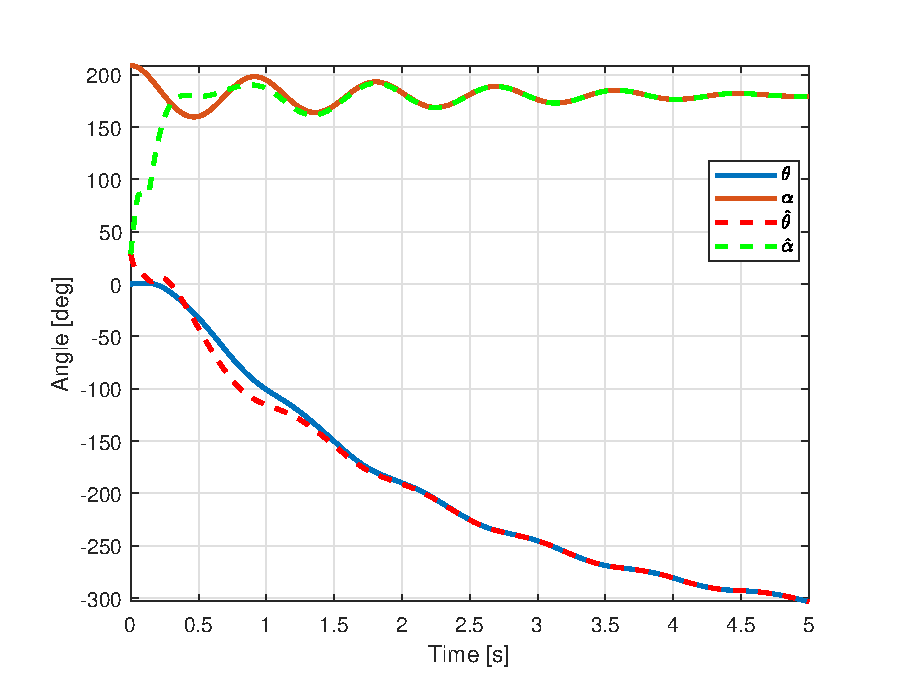
\includegraphics[width = \linewidth]{swingFailPos.eps}
                \caption{Non-linear estimator converging to true state angular position during a failed swing up.}
                \label{fig:swingFailPos}
            \end{figure}
        }
    }
    \section{Conclusion}
    {
        This report has focused on five sections. Section 1 introduces the chosen topic. Section 2 then explains about the system. Continuing on, section 3 discusses the details of system modelling and moves into section 4 where system linearization was constructed. Finally, in section 5 controller design and simulations were simulated using Matlab Simulink and was explained better using graphs. The report is then summarized into a conclusion which is as explained.

        In conclusion, this report presents an in-depth analysis on a designed process of controllers for an inverted rotary pendulum. The system was modelled using the lagrangian formulation of mechanics to develop a non linear model. It was then linearized at an equilibrium point to achieve space state matrices. This process was followed by designing a swing up controller. To evaluate the performance of the controller, the closed-looped system was tested.  However it did not produce the expected results. Even though it was able to bring the pendulum to a vertical position, an unexpected behaviour was achieved. With an addition of the non-linear observer, the swing up system had caused a failure in simulation. This was due to the convergence error. To eliminate this issue, other solvers such as ODE45 were used. Although it did produce a plot, an absence in the swing up action was observed. This might have occurred as a result of the non-linear nature of the swing up controller. Therefore, a further investigation is needed, to identify in order to solve this issue. This proposed method could be a promising approach used for non-linear control systems in general. 


        All files used for this project can be found at \url{https://github.com/ankithadas/Design-Project2.git}.
    }
    \bibliography{MyRefs}
    \bibliographystyle{IEEEtran}
\end{document}